The square wave generator functionality of the RTC can be utilised when the
interrupt bit is set low. The output of the square wave generator can be one of
four predetermined values, as indicated in Figure \ref{fig:images-sqWave}.

\begin{figure}[H]
	\centering
	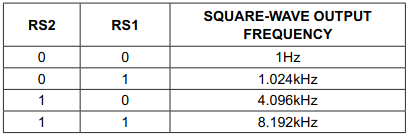
\includegraphics[width=0.8\textwidth]{images/sqWave}
	\caption{Square Wave Generator Frequency}
	\label{fig:images-sqWave}
\end{figure}

The ``sqWaveGen'' function, shown in Listing \ref{lst:sqWave} was implemented in order
to set the frequency of the square wave generator output. This function takes an
integer value input, representing the four available frequency outputs, and sets
the values of the Rate Select bits based on this input.

\lstinputlisting[language={C++}, caption={sqWaveGen Function},label={lst:sqWave}]
{snippets/sqWave.cpp}

A switch statement is used in order to set or clear the bits in the desired
positions, using the changeBits function. Once the switch statement exits, the
writeToReg function is used to write the new value in the buffer to the
register.
